%\setcounter{section}{0}
%\setcounter{subsection}{0}
%\setcounter{subsubsection}{0}
%\setcounter{equation}{0}
%\pagenumbering{arabic} 
%\setcounter{page}{0}    %%%%%KKD used \setcounter{page}{0}  
%\oddsidemargin 0.9 cm 
%\evensidemargin -.4 cm
%\setlength{\textwidth}{152.4 mm}
\chapter{Summary and Conclusion  \label{ Summary and Conclusion}}

We presented our studies on three different topics. The first two being the two search analysises in SUSY and one search on Leptoquark. We did not see any evidence of new physics in any of our studies . But the limits are considerably extended from the previous 8TeV studies. Here we compare the upper limits on the cross section just from one channel with four top quark in the final state. We see that the upper limit for zero LSP mass hypothesis has been extended from around 1200 GeV to 1600 GeV with a small amount of 13 TeV data. We have not showncomparison plots from four light quark and four b quark final states but all the plots including the 8TeV and 13 TeV could be found from the CMS twiki page for supersymmetry public results here in Ref.~\cite{CMSSUSPublic}. More ever in 2016 analysis with 12.9 $\rm fb^{-1}$ of data , we extended the 2.3 $\rm fb^{-1}$ limits considerably. 

\begin{figure}[h]
\centering
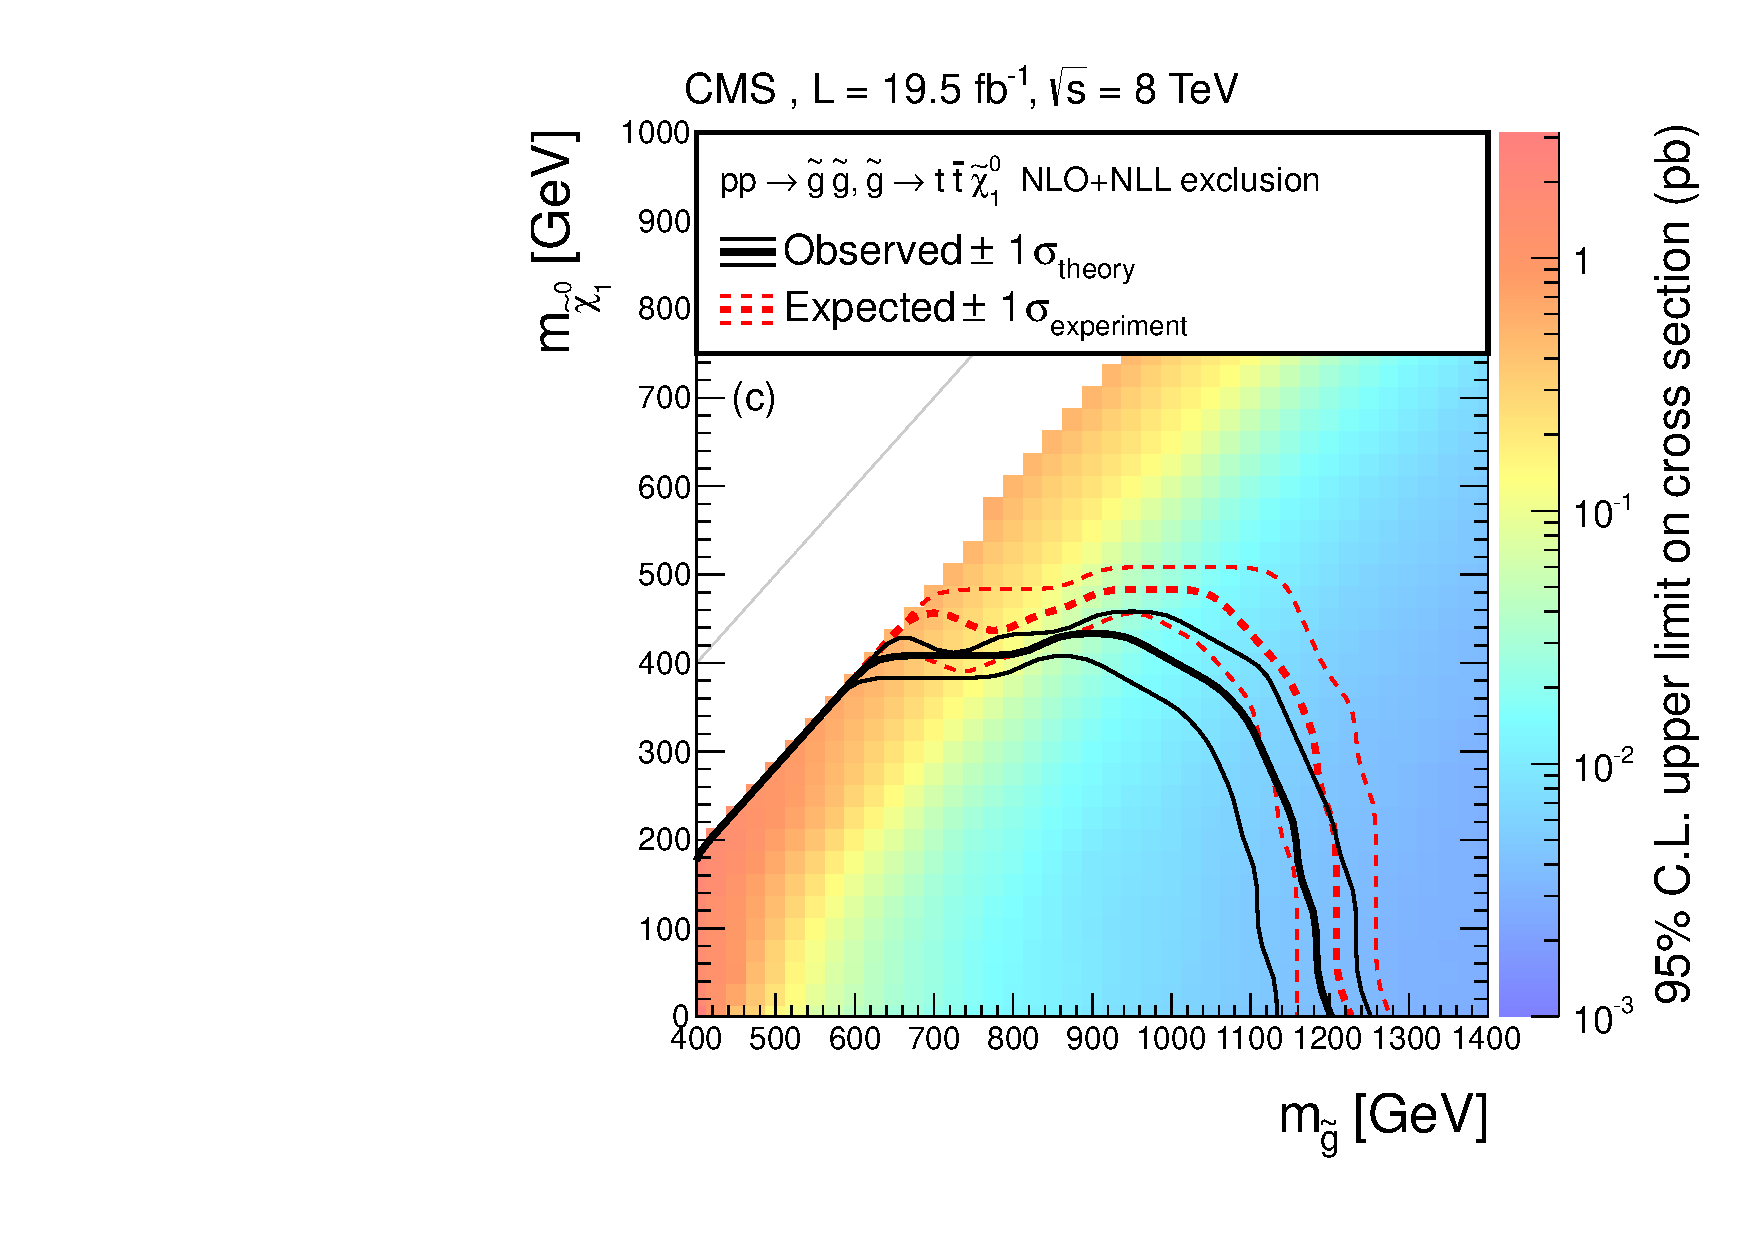
\includegraphics[width=0.42\textwidth]{/home/bibhu/Desktop/PhDThesis/PhDThesis/chapter9/CMS-Limit8TeVT1tttt.pdf}
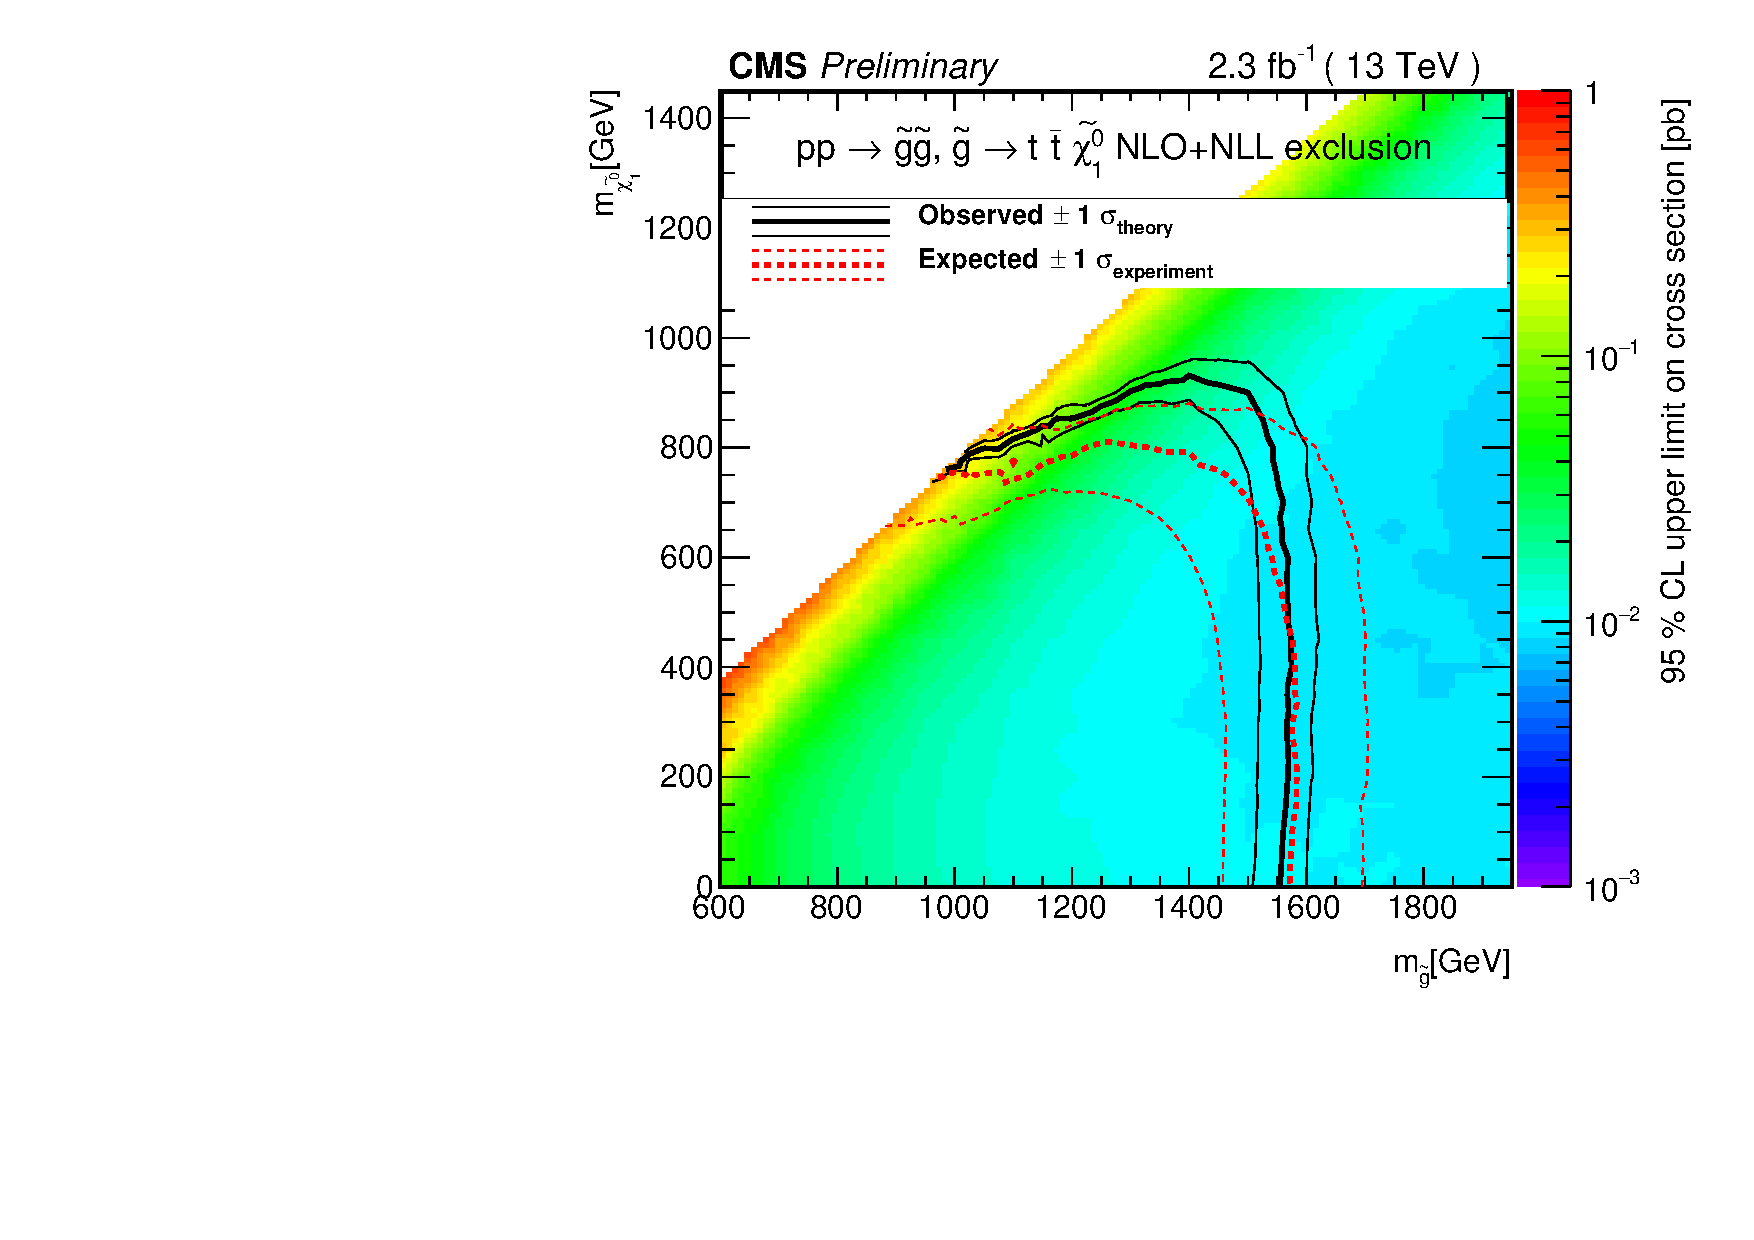
\includegraphics[width=0.47\textwidth]{/home/bibhu/Desktop/PhDThesis/PhDThesis/chapter9/T1tttt_2p3_limit.pdf}
\caption{\label{fig:Limit2016}The 95\% CL upper limits on the gluino pair production cross sections for four top quark final state. The left plot is taken from Ref.~\cite{SUSYhad8TeV}. The right plot is produced by us with 2.3 $\rm fb^{-1}$ of data.}
\end{figure}


Similarly in the Leptoquark analysis we have also extended the previous limits. But the limits are not improved as much as in SUSY because the increase in cross section in SUSY in much higher going from 8TeV to 13 TeV as compared to the LQ models. Here we present a comparison of the 8TeV limit vs the 13 TeV limits. More ever a small excess was seen for LQ mass 650 GeV in the 8TeV analysis ~\cite{CMS-PAS-EXO-12-041} but we did not see that excess confirming the prior could be a statistical fluctuation.

\begin{figure}[h]
\centering
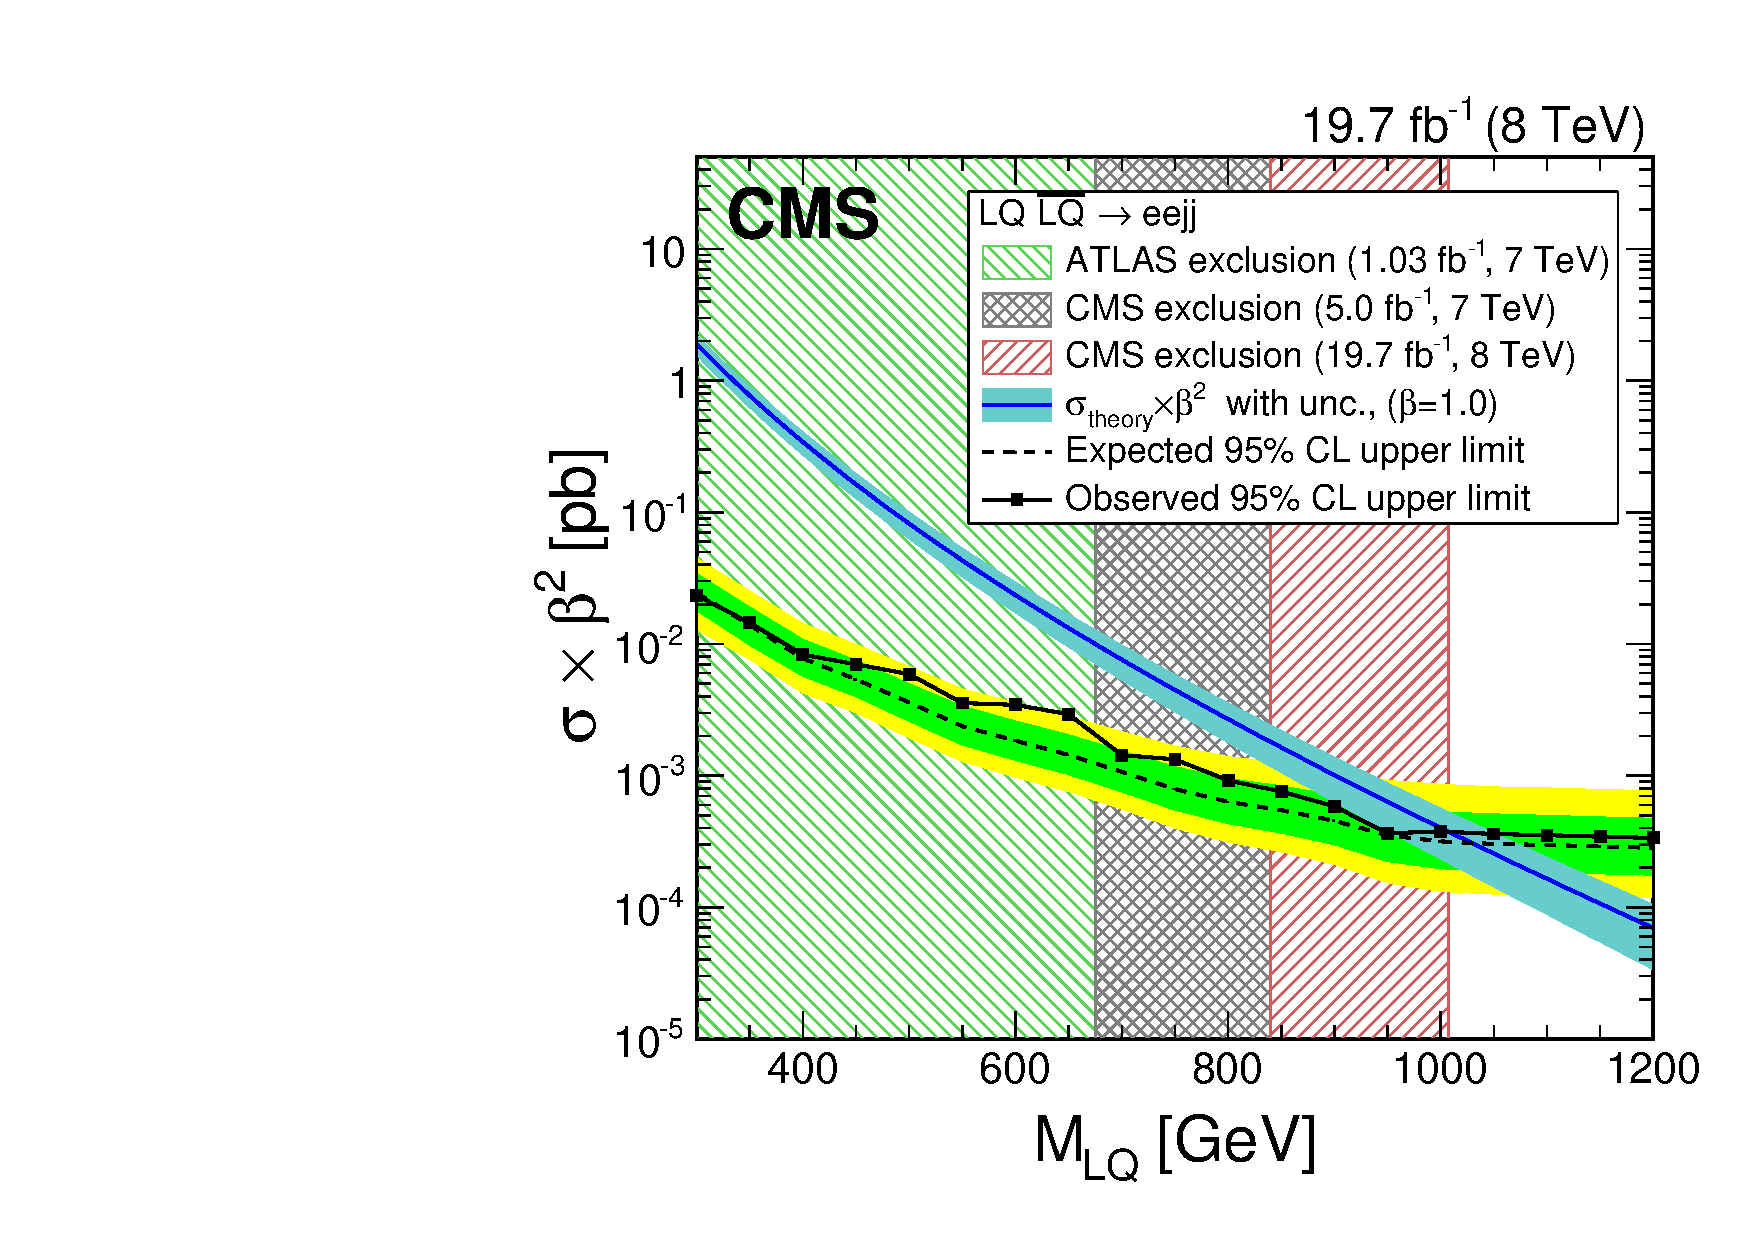
\includegraphics[width=0.42\textwidth]{/home/bibhu/Desktop/PhDThesis/PhDThesis/chapter9/LQ18Tevlimit.pdf}
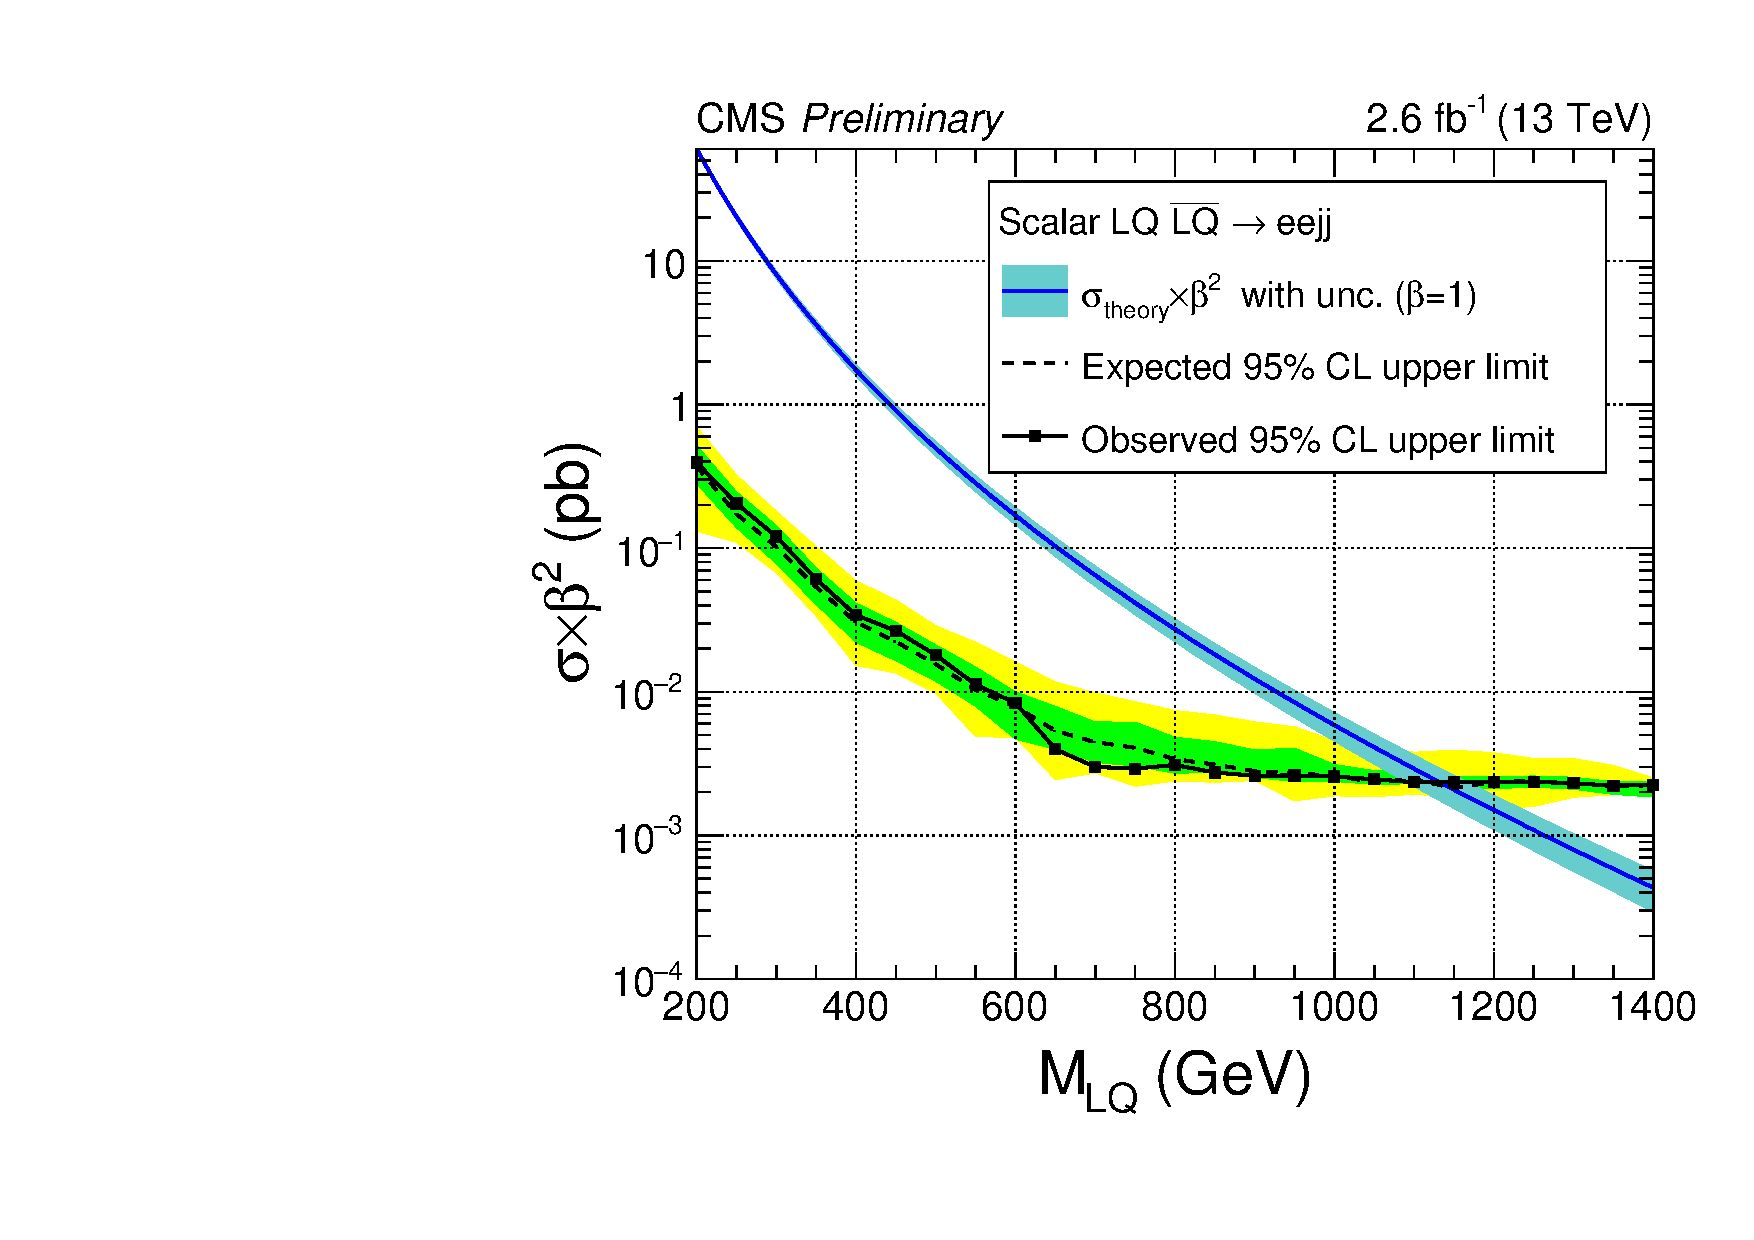
\includegraphics[width=0.42\textwidth]{/home/bibhu/Desktop/PhDThesis/PhDThesis/chapter9/LQLimitPlot.pdf}
\caption{\label{fig:LQLimit8TeV13TeV}The 95\% CL upper limits on the lepto quark production cross section . The left plot is taken from Ref.~\cite{CMS-PAS-EXO-12-041}. The right plot is produced by us with 2.6 $\rm fb^{-1}$ of data.}
\end{figure}


At the end we presented a study on the grooming techiniques. The grooming techniques becomes very useful when jets are contaminated with pileup. Many of the CMS analysises are using grooming techiques in their analysis now.

With this we colclude the presentation of the work that has been carried out during my PhD.
































